\documentclass{article}
\usepackage{hyperref}
\usepackage{graphicx}
\usepackage{siunitx}
\begin{document}
\section{DECAM Information}
From the DECam Imager Handbook: \newline
\begin{figure}[hbt!]
    \centering
    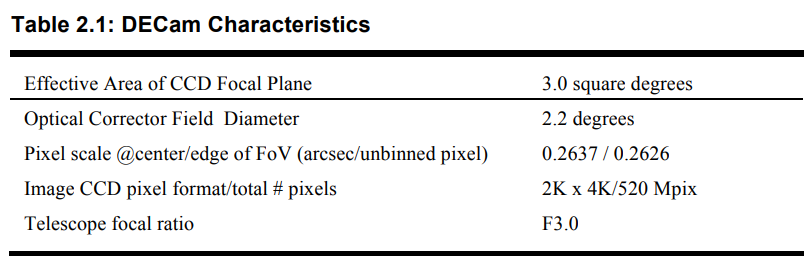
\includegraphics[width=0.5\linewidth]{Decam Characteristics.png}
    \caption{DECam Characteristics}
    \label{fig:enter-label}
\end{figure}
DECam has a three square degree field of view (2.2 degrees wide). It images at a resolution of 0.263 arcseconds per pixel. In particular, 0.2637 arcsec/pixel (center), 0.2626 arcsec/pixel (edge).  0.2637/0.2626 (arcsec/unbinned pixel). S Large focal plane array with a close to circular array of 62 CCDs and a total of 520 million pixels. 
\newline 
CCD Array Characteristics:
\newline
Array Dimensions: 
    Axis 1: 2048 pixels
    Axis 2: 4096 pixels
\newline
Pixel Size: \SI{15}{\micro\metre}

We are looking to use \textbf{resampled} images that have a zero-point associated with them. In the astro data archive, this corresponds to files with the process type (\texttt{proc_type}) of \texttt{resampled}, and the presence of the \texttt{MAGZERO} and/or \texttt{MAGZPT} fields.

\texttt{MAGZERO} data field: The (astronomical) magnitude corresponding to a single photon count in the image. This is located in the \textit{Extension} headers of the FITS files, present in Level 2 data products (single, reduced exposures). (From the DECam data handbook)\\

\section{Declination Range of the 2.3m Telescope}
\href{https://www.cambridge.org/core/journals/publications-of-the-astronomical-society-of-australia/article/anu-wifes-supernova-programme-awsnap/1DF292200162D34D6E5A268CE18C3653} {Physical Pointing Limit of the 2.3m}
\begin{figure}[hbt!]
    \centering
    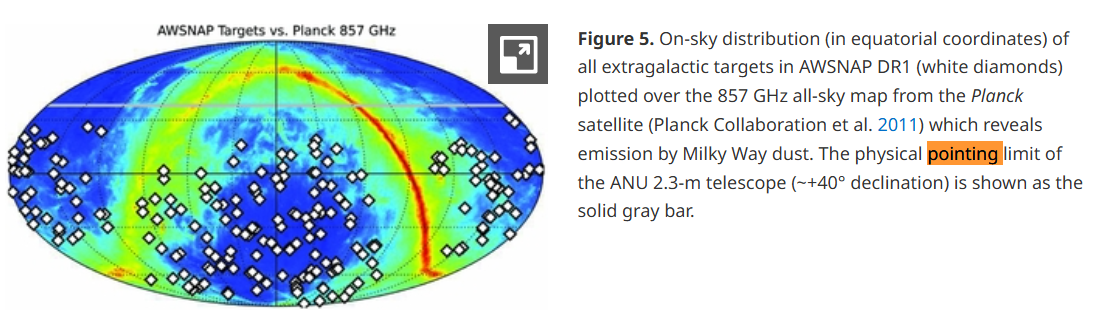
\includegraphics[width=0.5\linewidth]{image.png}
    \caption{Enter Caption}
    \label{fig:enter-label}
\end{figure}

\begin{figure}
    \centering
    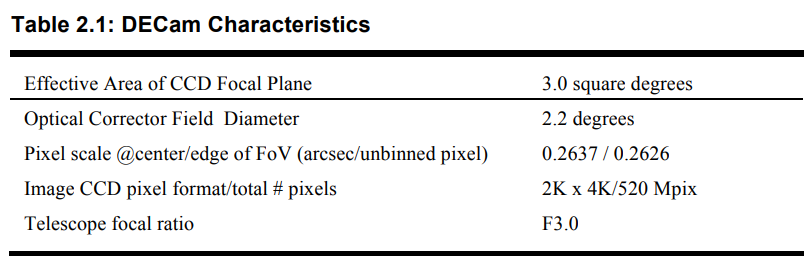
\includegraphics[width=0.5\linewidth]{Decam Characteristics.png}
    \caption{DECam Characteristics}
    \label{fig:enter-label}
\end{figure}

  \section{link dump}

  \href{https://github.com/cyb0rb/WiFeS_Catalog}{github repo}
  
  \href{https://sep.readthedocs.io/en/v1.1.x/tutorial.html}{source extractor tutorial}

\subsection{DECam}
  \href{https://astroarchive.noirlab.edu/api/docs/}{NOIRLab astro data archive}

  \href{https://github.com/NOAO/nat-nb/blob/master/sia.ipynb}{data archive query example notebook}

  \href{https://www.darkenergysurvey.org/the-des-project/data-access/}{DES project data access}

  \href{https://noirlab.edu/science/sites/default/files/media/archives/documents/scidoc0436.pdf}{DECam imager data handbook}
  
  \href{https://noirlab.edu/science/programs/ctio/instruments/Dark-Energy-Camera}{NOIRLab DECam information page} (has more links)
  
  \href{https://des.ncsa.illinois.edu/releases/other}{DES Data Management}

  \href{https://aus01.safelinks.protection.outlook.com/?url=https}{2.3m projects}
\end{document}